\section{Aufbau}

\begin{figure}[H]
  \centering
  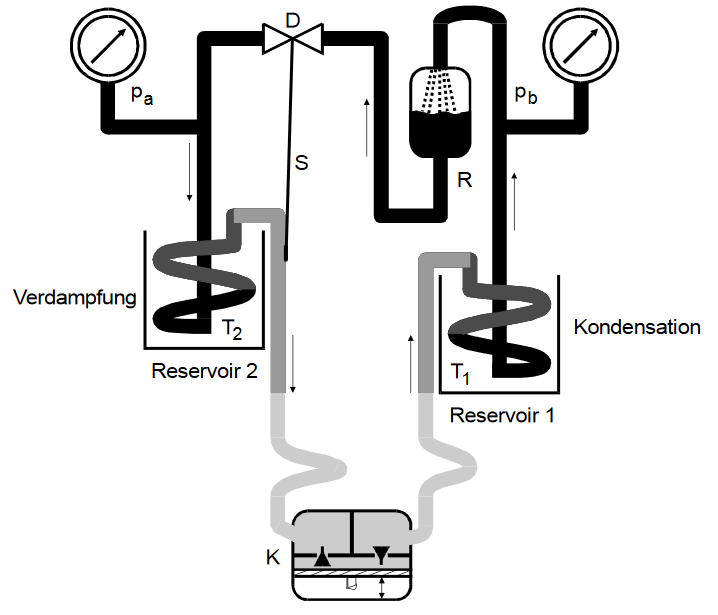
\includegraphics[height=8cm]{Waermepumpe.PNG}
  \caption{Aufbau der Wärmepumpe.}
  \label{fig:plot}
\end{figure}

Die Wärmepumpe besteht aus zwei Wärmereservoiren die über ein isoliertes
Rohr miteinander verbunden sind. In diesem befindet sich ein Gas, welches
durch das Einschalten eines in den Kreislauf integrierten Kompressors zu strömen
beginnt.\\
Zwischen den Teilen der Gasleitung, die die Wärmereservoire durchlaufen,
ist dabei ein Drosselventil eingebaut, welches einen Druckunterschied $p_b-p_a$
in der Leitung erzeugt. Dieser sorgt dafür, dass das Gas beim Durchlaufen
des einen Reservoirs kondensiert und, sobald es das Drosselventil passiert,
wieder verdampft. Nach dem Durchlaufen des zweiten Reservoirs wird es anschließend im Kompressor noch
weiter komprimiert, bevor es dann wieder in den Teil des ersten Reservoirs gelangt.
Das Gas nimmt beim Verdampfen Wärmeenergie auf und gibt sie beim Kondensieren
dann wieder ab. Somit wird die Wärme in Form von Phasenumwandlungsenergie transportiert.
Es ist daher sinnvoll ein Gas mit einer möglichst hohen Verdampfungswärme $L$
zu verwenden.

\label{sec:Aufbau}
